\documentclass{article}
\usepackage[utf8]{inputenc}
\usepackage[margin=2cm]{geometry}
\usepackage{fullpage,enumitem,amssymb,amsmath,xcolor,cancel,gensymb,hyperref,graphicx}
\usepackage{indentfirst}

\hypersetup{hidelinks} 

% \hypersetup{
% colorlinks=true,
% linkcolor=black
% }

\setlength{\parskip}{1em}

\title{EE6129 Assignment \uppercase\expandafter{\romannumeral2}}
\author{\bf{Ding Bangjie} \\
\\
G2001686F \\
\\
ding0130@e.ntu.edu.sg}
\date{}

\begin{document}

\maketitle

\section{Problem 1}
\subsection*{SOLUTION:}
\subsubsection*{a)}
\par From the description of the problem, it is a \textbf{8-QAM} modulate.
\par The modulated waveform function can be expanded as:

\begin{equation}\label{eq:1}
 A_i\sin(\frac{2\pi}{T}t + \phi_j) = A_i\cos(\phi_j)\underline{\sin(\frac{2\pi}{T}t)} + A_i\sin(\phi_j)\underline{\cos(\frac{2\pi}{T}t)}
\end{equation}

\par The underlined terms come from the basis functions. Since it's QAM modulation, two basis function should be orthonormal. Can be expressed as following:

\begin{equation}\label{eq:2}
\int_{t=0}^T\Psi_i(t)\Psi_j(t)\mathrm{d}t = \left\{  
\begin{aligned}
1 \quad i = j \\
0 \quad i \neq j
\end{aligned}
\right.  
\end{equation}

\par Using the underlined term in formula.\ref{eq:1} we can get:
\begin{equation}\label{eq:3}
\begin{split}
\int_{t=0}^{T}\sin^{2}(\frac{2\pi}{T}t) \mathrm{d}t = & \int_{0}^{T}\frac{1}{2}(1-\cos(\frac{4\pi}{T}t))  \\
= & \frac{1}{2}(t - \frac{T}{4\pi}\sin(\frac{4\pi}{T}t))\bigg|_{0}^{T} \\
= & \frac{T}{2}
\end{split}
\end{equation}

\par Similarly, 
\begin{equation}\label{eq:4}
\int_{t=0}^{T}\cos^{2}(\frac{2\pi}{T}t) \mathrm{d}t = \frac{T}{2}
\end{equation}

\par Moreover,
\begin{equation}\label{eq:5}
\begin{split}
\int_{t=0}^{T}\sin(\frac{2\pi}{T}t)\cos(\frac{2\pi}{T}t)\mathrm{d}t = & \bigg[\frac{T}{4\pi}\sin^{2}(\frac{2\pi}{T}t) + C\bigg] \bigg|_{0}^{T} \\
= & 0  
\end{split}
\end{equation}


\par In order to meet the condition in formula.\ref{eq:2}, the results of formula.\ref{eq:3} and \ref{eq:4} must be $1$, therefore, we add a constant in the underlined terms from the formula.\ref{eq:1} without changing the result of formula.\ref{eq:5}.

\par We conclude that the basis function of this modulated signal is:
$$ \Psi_1(t) = \sqrt[]{\frac{2}{T}}\sin(\frac{2\pi}{T}t) $$
$$ \Psi_2(t) =\sqrt[]{\frac{2}{T}}\cos(\frac{2\pi}{T}t) $$


\subsubsection*{b)}
\par As described in the problem, 1 of the 3 bits is carried in the amplitude $A_i$ and the remaining 2 bits are carried in the phase $\phi_j$. It can be considered as QPSK with 2 different amplitudes.

\par The constellation of 8-QAM is showed in figure.\ref{fig:8-QAM}\footnote{This figure is edited based on the QPSK constellation diagram generated by MATLAB Communication Toolbox. The source code is available on my github homepage.}.

\begin{figure}[!h]
\centering
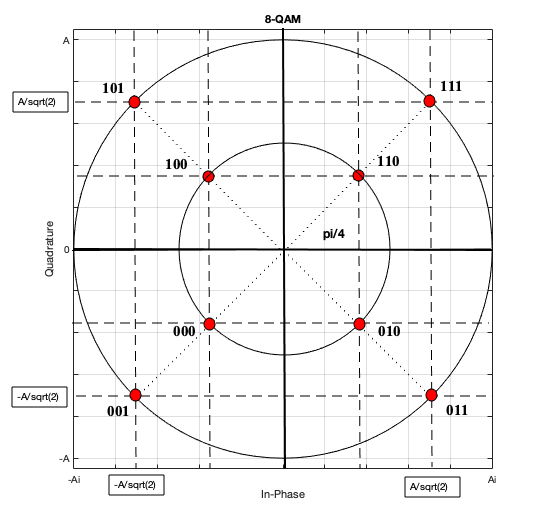
\includegraphics[scale=0.5]{./figure/QAM_8_1}
\caption{The constellation diagram of 8-QAM with initial phase $\frac{\pi}{4}$.}
\label{fig:8-QAM}
\end{figure}

\par This modulation uses 2 possible amplitudes and 4 possible phases. In 8-QAM, the duration of a symbol is three times the duration of a bit (since each symbol carries 3 bits). There are both phase and amplitude changes for each symbol. For the constellation shown above, the eight output symbols might be:
\begin{equation}
\begin{split}
& A\cos(2\pi f_c t \pm \frac{\pi}{4}) \\
& A\cos(2\pi f_c t \pm \frac{3\pi}{4}) \\
& \frac{A}{2}\cos(2\pi f_c t \pm \frac{\pi}{4}) \\
& \frac{A}{2}\cos(2\pi f_c t \pm \frac{3\pi}{4}) 
\end{split}
\end{equation}

\par  Labeled using gray code where only one bit changes between adjacent coordinates. Gray code is used to minimize the number of bits that could be received in error. Besides, using $11\mathrm{X}, 10\mathrm{X}, 00\mathrm{X}, 01\mathrm{X}$ indicate phase in $\frac{\pi}{4},\frac{3\pi}{4},-\frac{3\pi}{4}, -\frac{\pi}{4}$ respectively. Similarly, using $\mathrm{XX}0, \mathrm{XX}1$ represent amplitude in $\mathrm{A},\mathrm{\frac{A}{2}}$. In this way, we get $8$ kinds of combinations with different phases and amplitudes.

\newpage
\section{Problem 2}
\subsection*{SOLUTION:}




\section{Additional Problem Set 1}


\end{document}
